%%%%%%%%%%%%%%%%%%%%%%%%%%%%%%%%%%%%%%
%%  NewMathTemplate.tex
%%  Template file for New Math Style
%%  MIT Press
%%  May 21,2016
%%  Written by Amy Hendrickson
%%  amykaren@mit.edu
%%%%%%%%%%%%%%%%%%%%%%%%%%%%%%%%%%%%%%

%% Please copy and rename this file to use when
%% starting your book.

%%%%%%%%%%%%%%%%%%%%%%%%%%%%%%%%%%%%%%%%%%%%%%%%%%%%%%%
%% Setting  Options

%% Choose size of your book: Consult your editor to
%% find which size you should use.
%% Choices are: [6x9], [7x9], [7x9wide], and [8x9]

\documentclass[6x9]{newmath}

%% In addition you can call for the manuscript option, for
%% double spacing:
%\documentclass[manuscript,6x9]{newmath}

%% Another option is `hyper'
%% to turn on the commands found in the hyperref package:
%\documentclass[hyper,6x9]{newmath}
% Information on hyperref commands found here:
% https://en.wikibooks.org/wiki/LaTeX/Hyperlinks
% 
% For package options and user commands:
% http://tug.ctan.org/tex-archive/macros/latex/contrib/hyperref/doc/manual.pdf
% 
% The hyperref package is entered at the very end of the newmath.cls
% file, in case you'd like to make changes to the package options.
% 
%%%%%%%%%%%%%%%%%%
% Cropmarks are used by default. If you  want to turn cropmarks off, type
% \nocropmarks (before \begin{document})

%%%%%%%%%%%%%%%%%
% Author definitions go before \begin{document}

% ie, \def\taupav{\tau_{\mathrm{Pav}}}

% It's better to put definitions in the body of your .tex file
% rather than having a separate file for your macros, which
% can become separated from your .tex file.

\begin{document}

%%%%%%%%%%%%%%%%%%%%%%%%%%%%%%%%%%%%%%%%%%%%%%%%%%%%%%%
%% Using Include 
%% Many authors set up their book using \include{}
%%

%% For instance:
% \include{front} %% containing all the front matter
% \include{chap1}
% \include{chap2}
% \include{chap3}
% \include{chap4}
% ...
% \endinput % end book here until ready to do endmatter
% \endnotes
% 
\begin{glossary}

% \rdv{We can just copy a big chunk of this from the FL MOOC.}

\term{Fidelity}{
The probability that a state matches another state, typically the state desired for that point in a computation.
}

%(Source: Riken Research:
%\url{http://www.rikenresearch.riken.jp/eng/frontline/5444})\\ 

\end{glossary}
% \bibliographystyle{mit-chicago}
% \bibliography{bibsamp}
% \printindex

%% Using \includeonly{chap1,chap3,etc.}
%% You can use \includeonly{} before \begin{document} to
%% include only the chapters you are presently working on.
%%%%%%%%%%%%%%%%%%%%%%%%%%%%%%%%%%%%%%%%%%%%%%%%%%%%%%%%%%%%%%%%%%%

%% This example does not use include. This front matter could
%% be in a separate file if you were using include

%\title{}
%\subtitle{}
%% optional
% \edition{}
%% author, or authors
%\author{}

%% ie
%\title{Economics of Industrial Ecology}
%\subtitle{Materials, Structural Change, and Spatial Scales}
%\edition{Second Edition}
%\author{Jeroen van den Bergh and Marco A. Jannsen}

%%%%%%%%%%%%%%%%%%%%%%%%%%%%%%%%%%%%%%%%%%%%%%%%%%%%%%%
%% makes half titlepage print, using info above
% \halftitlepage

%%%%%%%%%%%%%%%%%%%%%%%%%%%%%%%%%%%%%%%%%%%%%%%%%%%%%%%
%% Series Page
% \begin{seriespage}
%  \seriestitle{}
%  \serieseditor{}

%% repeat often as needed
%  \title{}
%  \author{}

%  \title{}
%  \author{}
%  \end{seriespage}

% ie,
%\begin{seriespage}
%\seriestitle{Industrial Economics}
%\serieseditor{Miriam Smith and Simon Rattle, editors}
%\title{Engineering and Economics}
%\author{Samuel Endgrove}
%\title{Structural Economics: From Beginning to End}
%\author{Guang Xi}
%\end{seriespage}

%%%%%%%%%%%%%%%%%%%%%%%%%%%%%%%%%%%%%%%%%%%%%%%%%%%%%%%
%% Make titlepage print, using info given above
% \titlepage

%%%%%%%%%%%%%%%%%%%%%%%%%%%%%%%%%%%%%%%%%%%%%%%%%%%%%%%
%% Copyright page

% \begin{copyrightpage}
% Copyright text here. 
% ISBN etc.
% \end{copyrightpage}

%%%%%%%%%%%%%%%%%%%%%%%%%%%%%%%%%%%%%%%%%%%%%%%%%%%%%%%
%% Dedication page
\dedication{}

% ie,
% \dedication{To our families, with gratitude,\\ ---JB and
% MJ} 

%%%%%%%%%%%%%%%%%%%%%%%%%%%%%%%%%%%%%%%%%%%%%%%%%%%%%%%
%% Optional Epigraph page, use as many epigraphs as you want

% \begin{epigraphpage}
% \epigraph{<text>}{<author>, source}

% \epigraph{<text>}{<author>, source}

% \end{epigraphpage}

%%%%%
% ie,
% \begin{epigraphpage}
% \epigraph{Begin at the beginning,'' the King said, gravely, ``Then
% go till you come to the end; then stop.''}{Lewis Carroll, {\it Alice
% in Wonderland}}

% \epigraph{You can never get a cup of tea large enough or a book long enough to
% suit me''}{C. S. Lewis}
% \end{epigraphpage}

%%%%%%%%%%%%%%%%%%%%%%%%%%%%%%%%%%%%%%%%%%%%%%%%%%%%%%%
%% Table of Contents, List of Figures, List of Tables
% \tableofcontents
%%% These lists are optional:
% \listoffigures
% \listoftables

%%%%%%%%%%%%%%%%%%%%%%%%%%%%%%%%%%%%%%%%%%%%%%%%%%%%%%%
%% Contributors list for edited book:

%\begin{contributors}
%\end{contributors}

%% Or, you may use the twocolumn option:
% \begin{contributors}[twocolumn]
% \end{contributors}

%% entries made with 
% \contrib 
% Name\\
% Department\\
% Affiliation\\
% City, State, Country

%%%%%
% ie.
%  \begin{contributors}[twocolumn]
%  \contrib 
%  Professor Alan Guth\\
%  Center for Theoretical Physics\\
%  Massachusetts Institute of Technology\\
%  Cambridge, Massachusetts, USA
%  
%  \contrib 
%  Professor Andrei Linde\\
%  Department of Physics\\
%  Stanford University\\
%  Stanford, CA, USA
%  \end{contributors}

%%%%%%%%%%%%%%%%%%%%%%%%%%%%%%%%%%%%%%%%%%%%%%%%%%%%%%%
%% Preface

%\begin{preface}
% <preface text>
% end with:
% \author{<author name>}
% \date{<date of preface>(month and year)}
% \end{preface}

% ie,
% \begin{preface}
% Here is a sample preface that we will usually see 
% before the beginning of the book.
% \author{T. Author}
% \date{May, 2016}
% \end{preface}

%%%%%%%%%%%%%%%%%%%%%%%%%%%%%%%%%%%%%%%%%%%%%%%%%%%%%%%
%% Part, partintro
%%
% \part[<optional short version of title for TOC>]
% {<part title>}

%% optional part introduction
%\begin{partintro}
% \partintrotitle{<text>}
%<text. Section heads will not be numbered>
%\end{partintro}

%%%%%%
%% ie
% \part[Environmental Policy Analysis]
% {Environmental Policy Analysis: Various Models for Material
% Flows in the Economy}
% \begin{partintro}
% \partintrotitle{This is an introduction to the part}
% Policy analysis may be divided into a number of subspecialities\ldots
% 
% \end{partintro}



%%%%%%%%%%%%%%%%%%%%%%%%%%%%%%%%%%%%%%%%%%%%%%%%%%%%%%%
%% Chapter Head

%% note: if you want to break a line in the title in the TOC,
%% add \string\\ where you want the line break

% \chapter[<optional short version for TOC>]
% {<chapter title>} %% may use \\ to break lines in chapter title
                  %% but remember to use [<short title>] without the \\

%% to send another version of chapter title to running head:
% \chaptermark{<another version of chapter title>}

%% If edited book:
% \chapterauthor{<author name>}

%% Optional one or more Epigraphs
%% The first quotation mark will be supplied, so don't type it in:
% \epigraph{<quote>''}
% {<author>}
% \epigraph{<quote>''}
% {<author>}

%% Optional abstract
% \begin{abstract}
% <text>
% \end{abstract}

%%%%%% 
%% ie
% \chapter[Environmental Policy Analysis with STREAM:\protect\\
% Equilibrium Model for Material Flows in the Economy]
% {Environmental Policy Analysis with STREAM: A Partial
% Equilibrium Model for Material Flows in the Economy}
% 
% \chaptermark{Environmental Policy Analysis with STREAM}
% 
% \chapterauthor{Hein Mannaerts}
% 
% \epigraph{What star falls unseen?''}{William Faulkner}
% \epigraph{All seats provide equal viewing of the universe.''}{Museum
% guide, Hayden Planetarium}
% 
% \begin{abstract}
% Commercial robots are shown to be an effective manufacturing tool, but
% some shortcomings are noted, particularly their lack of mobility.
% \end{abstract}

%%%%%%%%%%%%%%%%%%%%%%%%%%%%%%%%%%%%%%%%%%%%%%%%%%%%%
% Section heads

% \section{<text>}
% \subsection{<text>}
% \subsubsection{<text>}
% \paragraph{<text>}

%%%%%%%%%%%%%%%%%%%%%%%%%%%%%%%%%%%%%%%%%%%%%%%%%%%%%
% Notation, show symbols or terms and then define them

% \begin{notation}
% <term>&<definition>\\
% <term>&<definition>\\
% <term>&<definition>\\
% ...
% \end{notation}

%%%%%%%
%% ie
% \begin{notation}
% $g_{\mu\nu}(x^\lambda)=g_{\nu\mu}(x^\lambda)$&symmetric tensor\\
% $g_{\mu\nu}\equiv\eta_{\mu\nu}=\mathrm{diag}(−1,1,1,1)$&Minkowski
% spacetime\\
% \end{notation}

%%%%%%%%%%%%%%%%%%%%%%%%%%%%%%%%%%%%%%%%%%%%%%%%%%%%%
% Note
%% The \note{} text will appear in the Notes section 
%% at the end of the chapter and/or the end of the book.
%% Remember to use the note at the end of a paragraph, 
%% not on its own line.


% \note{<text here>}

%%%%%%%%%%%%%%%%%%%%%%%%%%%%%%%%%%%%%%%%%%%%%%%%%%%%%
% Extract

% \begin{extract}
% <text>
% (<author of extract, where published, optional url>)
% \end{extract}

%%%
% ie

% \begin{extract}
% The distance $ds$ between two neighboring events, one with coordinates...
% (Kostas D. Kokkotas, Article for the Encyclopedia of Physical Science
% and Technology, 3rd Edition, Volume 7, Academic Press, (2002)
% \url{http://www.tat.physik.uni-tuebingen.de/~kokkotas/Teaching/NS.BH.GW_files/GW_Physics.pdf})
% \end{extract}

%%%%%%%%%%%%%%%%%%%%%%%%%%%%%%%%%%%%%%%%%%%%%%%%%%%%%
% Boxed Text
% Will continue over pages; may contain section heads, extracts, equations, theorems, 
% programming code, algorithms, etc.
% within the box. May use empty argument if you don't want title: \begin{boxedtext}{}...\end{boxedtext}

%\begin{boxedtext}{<title>}
% <text>
% optional attribution:
%(author, where published, \url{})
%\end{boxedtext}

%%%%
% ie

%\begin{boxedtext}{Frank Wilczek on Einstein and Gravitation}
%...
% (Frank Wilczek, Physics Today, April 2016,
% \url{scitation.aip.org/content/aip/magazine/physicstoday/article/69/4/10.1063/PT.3.3137})
% \end{boxedtext}

%%%%%%%%%%%%%%%%%%%%%%%%%%%%%%%%%%%%%%%%%%%%%%%%%%%%%
% Programming Code; 
% either \begin{code}\begin{verbatim}...\end{verbatim}\end{code} or
% \begin{algorithm}\caption{<text>}
% \begin{algorithmic}...\end{algorithmic}
% \end{algorithm}

% \begin{code}
% \begin{verbatim}
% <code here>
% \end{verbatim}
% \end{code}

%% or \begin{algorithm}...\end{algorithm}
%% See https://en.wikibooks.org/wiki/LaTeX/Algorithms for examples
%% http://tug.ctan.org/macros/latex/contrib/algorithms/algorithms.pdf

%%%%%
%% ie

%% (\begin{algorithm} takes option [p][b][t][h],  or some combination, like \begin{figure})
% \begin{algorithm}[h]
% \caption{A sample in an algorithm environment.}
% \begin{algorithmic}
% \If {$i\geq maxval$}
%     \State $i\gets 0$
% \Else
%     \If {$i+k\leq maxval$}
%         \State $i\gets i+k$
%     \EndIf
% \EndIf
% \end{algorithmic}
% \end{algorithm}

%%%%%%%%%%%%%%%%%%%%%%%%%%%%%%%%%%%%%%%%%%%%%%%%%%%%%
%% Outline, see NewMathSample for an example.
%% Use \begin{outline}...\end{outline};
%% Use enumerate for each level, use \item[<symbol>] for each item:

% \begin{outline}

% \begin{enumerate}
% \item[I.]
% <text>
% 
% \item[II.]
% <text>
% 
% \begin{enumerate}
% \item[A.]
% <text>
% 
% \begin{enumerate}
% \item[1.]
% <text>
% 
% \item[2.]
% <text>
% \end{enumerate}
% 
% \item[B.]
% <text>
% 
% \item[III.]
% <text>
% 
% \end{enumerate}

% \end{outline}


%%%%%%%%%%%%%%%%%%%%%%%%%%%%%%%%%%%%%%%%%%%%%%%%%%%%%
% Dialogue

% \begin{dialogue}
% \speaker{<name>}
% <Text>
% \speaker{<name>}
% <Text>
% \speaker{<name>}
% <Text>
% \end{dialogue}

%%%%%
%% ie
% \begin{dialogue}
% \speaker{France C\'ordova}
% It’s been decades, through a lot of different technological innovations...
%
% \speaker{Janna Levin}I was freaking out!
% 
% \speaker{Robert Garisto} [the editor of Physical Review Letters] 
% I got goose bumps while reading the LIGO paper.
% \end{dialogue}

%%%%%%%%%%%%%%%%%%%%%%%%%%%%%%%%%%%%%%%%%%%%%%%%%%%%%
% Figure: illustration above, caption below, cross referencing \label{}
% within or after caption, not before it.

% \begin{figure}[t]
% <illustration here>
% \caption[<optional text to go to List of Figures>]
% {<text of caption>}
% \end{figure}

%%%%%%%%%%%%%%%%%%%
%% Landscape Figure

% \begin{figure}[p]
% \rotatebox{90}{\hskip<dimen> %to position figure vertically
% \vbox {\includegraphics[width=\textheight]{<file name>}
% \caption{<caption text}
% }%% <== end \vbox
% }%% <== end \rotatebox
% \end{figure}

% For instance,
% \begin{figure}[p]
% \rotatebox{90}{\hskip-3in\vbox {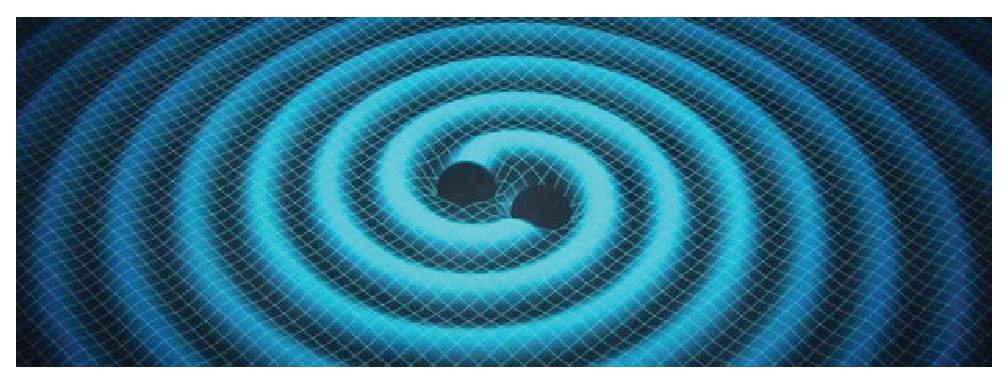
\includegraphics[width=\textheight]{gravwaves}
% \caption{(landscape figure)
% Graphic showing two black holes generating gravity waves.}}}
% \end{figure}



%%%%%%%%%%%%%%%%%%%%%%%%%%%%%%%%%%%%%%%%%%%%%%%%%%%%%
% Table: caption above, table below. Cross-referencing \label{}
% within or after caption, not before it.

% \begin{table}
% \caption[<optional text to go to List of Tables>]
% {<text of caption>}

% Optional centering, often used:
% \centering
% \begin{tabular}{lc}
% \hline
% Column Heads  \\
%\hline
% (table lines)(optional table note marker)$^a$\\
%\hline
% Optional table note in last line of table:
%\multicolumn{2}{l}{$^{a}$Table note text here.}
%\end{tabular}
%\end{table}

%%%%%%%%%%%%%%%%%%%%%%%%%%%%%%%%%%%%%%%%%%%%%%%%%%%%%
%% Using tabular in text: put in \blankline before
%% and after tabular. This will keep the table flush
%% left and keep the text following the table from indenting.

%%%%%
%% ie

% text...
% \blankline
% \begin{tabular}{rlcc}
% \hline
% &&\multicolumn2c{$Y$= Decrease in Surface Tension}\\
% \multicolumn2c{$x$ = Weight \% sulfur}
% &\multicolumn2c{(dynes/cm), two Replicates}\\
% \hline
% 0.&034&301&316\\
% 0.&093&430&422\\
% 0.&30&593&586\\
% \hline
% \end{tabular}
% \blankline
% text...

%%%%%%%%%%%%%%%%%%%%%%%%%%%%%%%%%%%%%%%%%%%%%%%%%
%% Landscape table

% \begin{table}[p]
% \rotatebox{90}{\vbox{
% \caption{<text>}
% \begin{tabular}{@{}crrrrrrrrrrr}
% ...
% \end{tabular}
% } <-- end vbox
% } <-- end rotate
% \end{table}

% For example,
% \begin{table}[p]
% \rotatebox{90}{\vbox{
% \caption{More relevant tabular information.\label{tbl-2}}
% \begin{tabular}{@{}crrrrrrrrrrr}
% \hline
% Star & Height & $d_{x}$ & $d_{y}$ & $n$ & $\chi^2$ & $R_{maj}$ & $R_{min}$ &
% \multicolumn{1}{c}{$P^a$} & $P R_{maj}$ & $P R_{min}$ &
% \multicolumn{1}{c}{$\Theta^b$} \\
% \hline
% 1 &33472.5 &-0.1 &0.4  &53 &27.4 &2.065  &1.940 &3.900 &68.3 &116.2 &-27.639\\
% 2 &27802.4 &-0.3 &-0.2 &60 &3.7  &1.628  &1.510 &2.156 &6.8  &7.5 &-26.764\\
% ...
% \hline\\
% \multicolumn{12}{l}{$^a$
% Sample footnote for table~\ref{tbl-2} that was
% generated with the \LaTeX\ table environment}\\
% \multicolumn{12}{l}{$^b$ Yet another sample footnote for table
% \ref{tbl-2}}\\
% \multicolumn{12}{l}{$^c$ Another sample footnote for
% table~\ref{tbl-2}}\\
% \end{tabular}}}
% \end{table}


%%%%%%%%%%%%%%%%%%%%%%%%%%%%%%%%%%%%%%%%%%%%%%%%%%%%%
%% Lining up decimal numbers on the decimal point:
%% For each decimal number, use two table columns; the
%% first pushing the text to the right, the second to the left.
%% to get rid of the space between the two columns, supply
%% @{}, as you see in the example below. See example in newmathsample.tex/.pdf
%% in exercise section.

% \begin{tabular}{r@{}lcc}
% \hline
% &&\multicolumn2c{$Y$= Decrease in Surface Tension}\\
% \multicolumn2c{$x$ = Weight \% sulfur}
% &\multicolumn2c{(dynes/cm), two Replicates}\\
% \hline
% 0.&034&301&316\\
% 0.&093&430&422\\
% 011.&30&593&586\\
% \hline
% \end{tabular}

%%%%%%%%%%%%%%%%%%%%%%%%%%%%%%%%%%%%%%%%%%%%%%%%%%%%
%% Continued Caption, \continuedcaption
%% Will work with tables And figures
%% 
%% It will give you ``Table <table number> (Continued)''
%% or ``Figure <table number> (Continued)''
%% The Table or Figure number will stay the same as the
%% previous table or figure.

% \begin{table}
% \caption{}
% \begin{tabular}{rlc}
% ...
% \end{tabular}
% \end{table}
% 
% \clearpage
% 
% \begin{table}
% \continuedcaption
% \begin{tabular}{rlc}
% ...
% \end{tabular}
% \end{table}
% 
%%  Or, for figures;
% 
% \begin{figure}
% <illustration>
% \caption{}
% \end{figure}
% 
% \clearpage
% 
% \begin{figure}
% <illustration>
% \continuedcaption
% \end{figure}

%%%%%%%%%%%%%%%%%%%%%%%%%%%%%%%%%%%%%%%%%%%%%%%%%%%%
% Longtable: Table that will continue over pages

% Long table needs these parts for the set up:

% 1) begin long table, give tabular preamble:
% \begin{longtable}{ccc@{}}

% 2) Supply caption and top of table with text preceding
% \endfirsthead

% \caption{ApJ costs from 1991 to 2013
% \label{tab:table}} \\[2pt]
% \hline
% \bf Year & \bf Subscription & \bf Publication \\
%  & \bf cost &\bf charges\\
%  & \bf(\$) & \bf (\$/page)\\
% \hline
% \endfirsthead

% 3) Supply continuation of table and column heads
% before the \endhead command:

% \multicolumn3c{\longtablecontinued}\\[7pt]
% \hline
% \bf Year & \bf Subscription & \bf Publication \\
%  & \bf cost &\bf charges\\
%  & \bf(\$) & \bf (\$/page)\\
% \hline
% \endhead

% 4) Supply extra space before footer at bottom of each page;
% ending with \endfoot.

% \\[12pt]
% \endfoot

% 5) Supply final ending to table with \hline and extra vertical space preceding
% \endlastfoot

% \hline
% \\[24pt]
% \endlastfoot

% 6) Type in table

% 7) End with this command:
% \end{longtable}

%%%%%%%%%%%%%%%%%%%%%%%%%%%%%%%%%%%%%%%%%%%%%%%%%%%%%%%%%%%%%%%
%% Citations done with NatBib

% Citations in the New Math book style are made using the Natbib
% commands. See table showing commands and results in NewMathSample
% or NewMathDocs.

% See \url{http://merkel.zoneo.net/Latex/natbib.php}
% for a reference sheet of natbib commands.

%%%%%%%%%%%%%%%%%%%%%%%%%%%%%%%%%%%%%%%%%%%%%%%%%%%%%%%%%%%%%%%%
%% End of Chapter

%%%%%%%%%%%%%%%%%%%%%%%%%%%%%%%%%%%%%%%%%%%%%%%%%%%%%%%%%%%%%%%%
%% Exercises

% \begin{exercises}
% \exer{}
% \subexer{}
% \sidebysidesubsubexer{}{}
% \end{exercises}

%%%%%
%  ie

% \begin{exercises}
% \exer{For Hooker's data, Exercise 1.2, use the Box and Cox and Atkinson procedures to determine a appropriate transformation of PRES
% in the regression of PRES on TEMP. find $\hat\lambda$, $\tilde\lambda$,
% the score test, and the added variable plot for the score. 
% Summarize the results.}

% \subexer{The following data were collected in a study of the effect of dissolved sulfur
% on the surface tension of liquid copper (Baes and Killogg, 1953).}

% \sidebysidesubsubexer{In the case of $\Delta_1$?}{In the case of $\Delta_2$?}

% \sidebysidesubexer{In the case of $\Gamma_1$?}{In the case of $\Gamma_2$?}
% \end{exercises}

%%%%%%%%%%%%%%%%%%%%%%%%%%%%%%%%%%%%%%%%%%%%%%%%%%%%%%%%%%%%%
%% Chapter Appendix

% \begin{chapappendix}{<title>}
% <text>
% \end{chapappendix}

%%%%%
%  ie
% \begin{chapappendix}{Dark Matter is not composed of Black Holes}

% \section{The Canada France Hawaii Lensing Survey}
% ...
% \end{chapappendix}

%%%%%%%%%%%%%%%%%%%%%%%%%%%%%%%%%%%%%%%%%%%%%%%%%%%%%%%%%%%%%
%% Chapter Notes: \chapternotes will make any \note{<text>} that
%% you entered in the chapter print, at the end of the chapter.

% \chapternotes

%%%%%%%%%%%%%%%%%%%%%%%%%%%%%%%%%%%%%%%%%%%%%%%%%%%%%%%%%%%%%
%% End of the Book

%%%%%%%%%%%%%%%%%%%%%%%%%%%%%%%%%%%%%%%%%%%%%%%%%%%%%%%%%%%%%
%% Appendix \appendix will make \chapter and \section use
%% letters rather than numbers. Also changes equation numbers
%% and figure and table numbers.

% \appendix
% \chapter{<title>}
% \section{<section head>}

%%%%%%%%%%%%%%%%%%%%%%%%%%%%%%%%%%%%%%%%%%%%%%%%%%%%%%%%%%%%%
% IMPORTANT:
% After Appendices, please enter
% \endmatter

% This command will give a little extra space in the Table of Contents
% before the Glossary and/or Bibliography, Index, other end of book 
% commands are printed.

%%%%%%%%%%%%%%%%%%%%%%%%%%%%%%%%%%%%%%%%%%%%%%%%%%%%%%%%%%%%%
%% Glossary

% \begin{glossary}
% \term{<term>}{<definition>}
% ...
% \end{glossary}

%%%%%
%  ie
% \begin{glossary}
% \term{Absolute Zero}{
% The lowest temperature possible, equivalent to -273.15°C (or 0° on the
% absolute Kelvin scale), at which point atoms cease to move altogether
% and molecular energy is minimal. The idea that it is impossible,
% through any physical process, to lower the temperature of a system to
% zero is known as the Third Law of Thermodynamics.}
% ...
% \end{glossary}

%%%%%%%%%%%%%%%%%%%%%%%%%%%%%%%%%%%%%%%%%%%%%%%%%%%%%%%%%%%%%
%% End Book Exercises / \exer{}, \subexer{}, \sidebysidesubexer{}{}
%% \sidebysidesubsubexer{}{} are the same as with exercises, only
%% \begin{endbookexercises}... \end{endbookexercises} is different
%%  at the end of the book.

% \begin{endbookexercises}
% \exer{}
% \subexer{}
% \sidebysidesubsubexer{}{}
% \end{endbookexercises}

%%%%%
%  ie

% \begin{endbookexercises}
% \exer{For Hooker's data, Exercise 1.2, use the Box and Cox and Atkinson procedures to determine a appropriate transformation of PRES
% in the regression of PRES on TEMP. find $\hat\lambda$, $\tilde\lambda$,
% the score test, and the added variable plot for the score. 
% Summarize the results.}

% \subexer{The following data were collected in a study of the effect of dissolved sulfur
% on the surface tension of liquid copper (Baes and Killogg, 1953).}

% \sidebysidesubsubexer{In the case of $\Delta_1$?}{In the case of $\Delta_2$?}

% \sidebysidesubexer{In the case of $\Gamma_1$?}{In the case of $\Gamma_2$?}
% \end{endbookexercises}

%%%%%%%%%%%%%%%%%%%%%%%%%%%%%%%%%%%%%%%%%%%%%%%%%%%%%%%%%%%%%
%% Endnotes: \endnotes will make every \note{<text>} that was entered
%% earlier in the book print here, with automatic sections for the
%% particular chapter built in. See NewMathSample.tex/pdf for example.

%\endnotes


%%%%%%%%%%%%%%%%%%%%%%%%%%%%%%%%%%%%%%%%%%%%%%%%%%%%%%%%%%%%%
%% Bibliography style should be mit-chicago, unless author
%% has strong preference for another style.

%%%%%
%  ie

% \bibliographystyle{mit-chicago}
% \bibliography{bibsamp}

%%%%%%%%%%%%%%%%%%%%%%%%%%%%%%%%%%%%%%%%%%%%%%%%%%%%%%%%%%%%%
%% Print Index

%\printindex

\end{document}
